\part*{Lektion 7: Vererbungen und Mehrfachvererbungen}
\section{Vererbung}
\begin{multicols}{2}
\begin{itemize}
	\item eine neue Klasse aus einer bestehenden Klasse ableiten:
	\item \textbf{Person} ist eine:
	\item[\-] Oberklasse, Basisklasse, Elternklasse oder Superklasse
	\item \textbf{Angestellter} und \textbf{Bürger} sind eine:
	\item[\-] Unterklasse, abgeleitete Klasse, Kindklasse oder Subklasse
\end{itemize}
\columnbreak
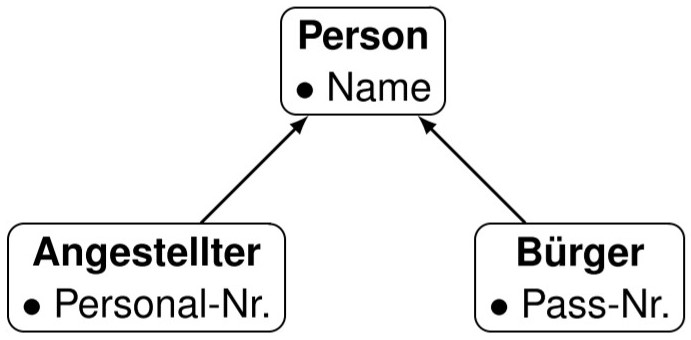
\includegraphics[width=0.8\linewidth]{images/v7_vererbung1}
\end{multicols}

\begin{itemize}
	\item Superklasse/Basisklasse:
	\item[\-] \lstinputlisting{listings/v7_vererbung1.py}
	\item Für die Vererbung: Superklasse in runden Klammern angeben
	\item Subklasse/abgeleitete Klasse:
	\item[\-] \lstinputlisting{listings/v7_vererbung2.py}
	\item Variablen und Methoden (\texttt{public} und \texttt{pretected}) werden direkt übernommen:
	\item[\-] \lstinputlisting{listings/v7_vererbung3.py}
	\item Methoden werden überschrieben, falls sie gleich heissen:
	\item[\-] \lstinputlisting{listings/v7_vererbung4.py}
	\item Zugriff auf die Superklasse mit \texttt{super()}
	\item[\-] \lstinputlisting{listings/v7_vererbung5.py}
\end{itemize}

\subsection{Beispiel}
\lstinputlisting{listings/v7_vererbung6.py}
Die Person-Klasse instanzieren:\\
\lstinputlisting{listings/v7_vererbung7.py}
Angestellte-Klasse erbt von der Person-Klasse:\\
\lstinputlisting{listings/v7_vererbung8.py}
Die Angestellter-Klasse instanzieren:\\
\lstinputlisting{listings/v7_vererbung9.py}

\subsection{\texttt{public}, \texttt{protected} und \texttt{private}}
Die Konvention ist wie folgt:
\begin{description}
	\item[\texttt{public:}] für für öffentliche Variablen und Methoden
	\item[\texttt{protected:}] (1 führender Unterstrich) für nicht-öffentliche Variablen und Methoden
	\item[\texttt{private:}] (2 führende Unterstriche) für nicht-öffentliche Variablen und Methoden, um Namenskonflikte in Subklassen zu vermeiden 
\end{description}
\url{https://www.python.org/dev/peps/pep-0008/#method-names-and-instance-variables}
\lstinputlisting{listings/v7_vererbung10.py}

\section{Mehrfachvererbung}
\begin{itemize}
	\item Eine Subklasse kann von mehreren Superklassen erben:
\end{itemize}
\begin{multicols}{2}
\lstinputlisting{listings/v7_vererbung11.py}
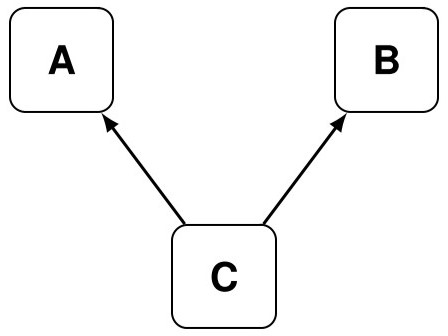
\includegraphics[width=0.7\linewidth]{images/v7_vererbung2}
\end{multicols}
Am besten die \texttt{\_init\_\(\)}-Methode der Klassen kooperativ machen, d.h.
\begin{itemize}
	\item immer \texttt{super()} benutzen
	\item Schlüsselwort-Argumente benutzen
	\item unbenutzte Schlüsselwort-Argumente weitergeben (\texttt{**kwargs})
\end{itemize}
\lstinputlisting{listings/v7_vererbung12.py}
\begin{multicols}{2}
\begin{itemize}
	\item \texttt{super()} ruft automatisch die Methode der nächsten Klasse auf
	\item Method Resolution Order (MRO) $\rightarrow$ C4 Superclass Linearization (\url{https://en.wikipedia.org/wiki/C3_linearizatio})
	\item Diamond-Problem ist kein Problem mit \texttt{super()}
\end{itemize}
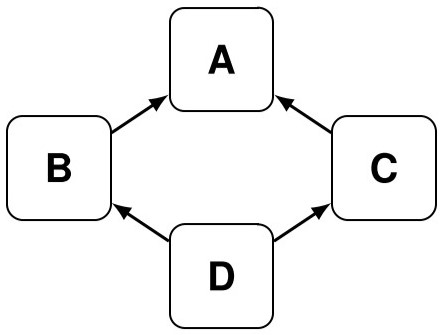
\includegraphics[width=0.5\linewidth]{images/v7_vererbung3}
\end{multicols}

\subsubsection{MRO}
Mehrfachvererbung in Diamant-Anordung:
\lstinputlisting{listings/v7_vererbung13.py}
\texttt{\textbf{super()}} ruft die Methoden der Reihe nach auf:
\lstinputlisting{listings/v7_vererbung14.py}
Die Reihenfolge wird vom MRO-Algorithmus festgelegt:
\lstinputlisting{listings/v7_vererbung15.py}
